\documentclass[xetex]{beamer}


\mode<presentation> {
  \usetheme{Frankfurt}
  \setbeamercovered{transparent}
}

\usepackage{xunicode}
\usepackage{xltxtra}
\usepackage[czech]{babel}
\usepackage{palatino}
\usepackage{graphicx}

\title{UNIX\\ základy}

\author{Ondřej Profant}
\institute[Piráti]{Knihovna Průhonice\\ Česká pirátská strana}
\date{\today}

\begin{document}
\begin{frame}
  \titlepage
\end{frame}

\begin{frame}
  \frametitle{Osnova}
  \tableofcontents
\end{frame}	

\begin{frame}
  \frametitle{}
  Dnes je význam nejasný, resp. mnohoznačný. 
  Většinou se myslí systém dle standardu POSIX. 
  Též se používá sousloví systém unixového typu (v angl. unix-like).
\end{frame}	

\section{Charakteristika}
\begin{frame}
  \frametitle{Charakteristika}
  \begin{itemize}
  \item víceuživatelský
  \item hierarchický souborový systém
  \item téměř vše je soubor
  \item plain text (prostý text) konfigurace
  \item orientovaný  na zpracování textu $\rightarrow$ shell
  \item manuálové stránky
  \item case sensitive (rozlišuje velikost písmen)
  \end{itemize}

Výsledek:
  \begin{itemize}
  \item jednoduchost
  \item univerzálnost
  \item tyto prvky se nezměnily od roku 1965
  \end{itemize}
\end{frame}	

\section{Systém souborů}
\subsection{Srovnání}
\begin{frame}
  \frametitle{Systém souborů - DOS}
  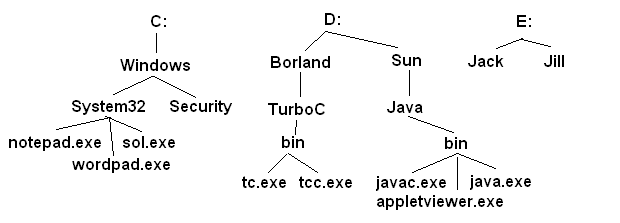
\includegraphics[scale=0.55]{pic/dosfs.png}
\end{frame}	

\begin{frame}
  \frametitle{Systém souborů - Windows}
  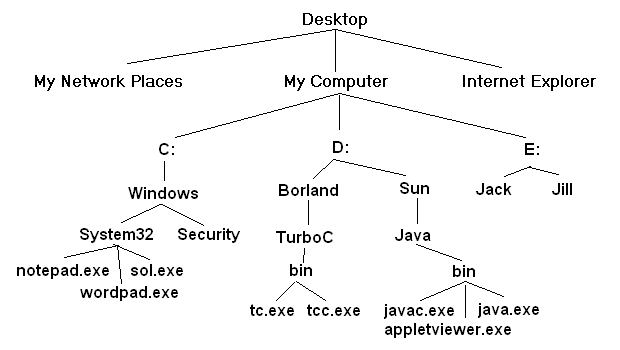
\includegraphics[scale=0.5]{pic/winfs.png}
\end{frame}	

\begin{frame}
  \frametitle{Systém souborů - UNIX}
  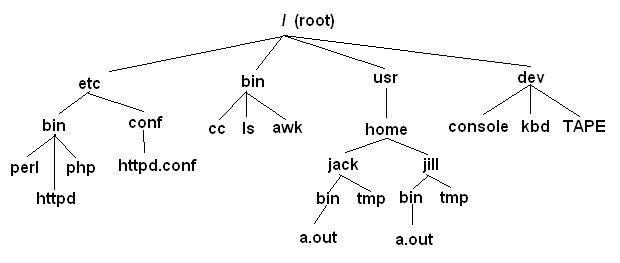
\includegraphics[scale=0.5]{pic/unixfs.png}
\end{frame}	

\subsection{Specifika}
\begin{frame}
  \frametitle{Systém souborů - UNIX}
  \begin{itemize}
  \item Nevyužívá se pouze jeden systém souborů
  \item Lze libovolně kombinovat (a běžně se to dělá)
  \item Skryté soubory začínají tečkou
 \end{itemize}
\end{frame}	

\section{Uživatelské účty}
\begin{frame}
  \frametitle{Uživatelské účty}
  \begin{itemize}
  \item silně využívány (více než ve světě Windows)
  \item každý uživatel má vše v adresáři \texttt{/home/<username>}
  \end{itemize}
\end{frame}	

\section{Shell}
\begin{frame}
  \frametitle{Shell}
  \begin{itemize}
  \item interakce s uživatelem (komunikace, ovládání)
  \item základní sada nástrojů
  \item tzv. ,,terminal''
  \item lze přes něj ovládat celý systém
  \end{itemize}
\end{frame}	

\subsection{Základní příkazy}
\begin{frame}
  \frametitle{Shell - základní příkazy 1}
  \begin{description}
  \item[man] zobrazení manuálové stránky
  \item[ls] obsah adresáře
  \item[mkdir] vytvoření adresáře
  \item[cat] zobrazení obsahu souboru
  \item[cp] kopírování souboru
  \item[mv] přesunutí souboru
  \item[grep] prohledání souboru pomocí regulární výrazů 
  \item[\ldots]
  \end{description}
\end{frame}	

\begin{frame}
  \frametitle{Shell - základní příkazy 2}
  \begin{description}
  \item[echo] vypsání argumentu (např. zobrazení zprávy)
  \item[find] hledání souborů (a nejen to)
  \item[sort] třídění
  \item[cut] vypsaní specifického sloupce
  \item[head] vypsání počátku
  \item[tail] vypsání konce
  \item[if, for, while] podmínky, cykly
  \item[\ldots]
  \end{description}
\end{frame}	

\begin{frame}
  \frametitle{Shell - práce s~příkazy}
  \begin{enumerate}
  \item Příkaz napíšeme do terminálu (popřípadě do skriptu). 
  \item Doplníme parametry.
  \item Můžeme ho zakončit středníkem. 
  \item Enter!
  \end{enumerate}
  
  Parametry jsou doplňující údaje, např. pokud chceme číst adresář i se skrytými soubory, tak zadáme:
  
  \texttt{ls --all --human-readable}
 
  Popřípadě obvykle lze parametry zkrátit:
  
  ls -a -h
  
  A zkrácené parametry lze i sloučit:
  
  ls -ah
\end{frame}	


\begin{frame}
  \frametitle{Shell - práce s~příkazy - pipe}
  Pipe (čti pajpa) je spojení dvou příkazů v jeden. Tam kde jeden příkaz končí, napojíme další.
  
  Například příkaz ls nám zobrazí obsah adresáře dle abecedy vzestupně, ale mi ho chceme mít seřazený sestupně. Inu na řazení je zde příkaz sort:
  
\texttt{ls | sort --reverse}
\end{frame}	

\subsection{Wildcards}
\begin{frame}
  \frametitle{Shell - wildcards}
  \begin{description}
  \item[*] 0-n znaků
  \item[?] jeden znak
  \item[[\ldots]] skupina znaků, např. [abc], [a-zA-Z], [0-9], [!0-9]
  \end{description} 
  Např: 
  \begin{description}
  \item[*.doc] všechny soubory končící koncovkou doc, např dokument.doc
  \item[zaloha?] najde např. zaloha1, zaloha2 etc., již ne zaloha10
  \end{description}
\end{frame}

\subsection{Vstupy a výstupy}
\begin{frame}
  \frametitle{Shell - vstupy a výstupy}
  Výstupy:
  \begin{description}
  \item[stdin] standardní vstup
  \item[stdout] standardní výstup
  \item[stderr] chybový výstup
  \end{description} 
  Přesměrování \texttt{cat file}:
  \begin{description}
  \item[1>] standardní vstup
  \item[2>] standardní výstup
  \item[\&>] oba výstupy
  \item[<] vstup
  \end{description}
  Např:
  
  \texttt{cat file > newfile}
  
  \texttt{grep pattern < file}
\end{frame}	

\begin{frame}
  \frametitle{Shell}
 Shellů je více druhů, dnes je nejrozšířenější BASH, avšak tyto základy jsou pro všechny stejné.
   \begin{description}
  \item[BASH] Born Again shell
  \item[DASH] Debian Almquist shell
  \item[CSH] C shell
  \item[KSH] Korn shell
  \item[\ldots]
  \end{description}
  Liší se rychlostí, bezpečností, velikostí, ale např. i prací s historii či inteligentním doplňováním. UNIXy si svobodně vybírají, který použijí. Dokonce shell u jednotlivých uživatelů se běžně liší.
\end{frame}	


\begin{frame}
 \frametitle{Bash - specifika}
 Doplňování pomocí tabulatoru.

 
 \end{frame}	

\begin{frame}
 Jste zmateni?
 
 To je zcela pochopitelné.
 
 \bigskip
 
 Pravá síla nastává až v kombinaci tohoto všeho napříč celým světem unixu.
\end{frame}

\begin{frame}
  \frametitle{Závěr}
	Děkuji za pozornost.

	\bigskip
	
	Doplňující otázky?

\bigskip

\bigskip

\scriptsize
Copyleft Ondřej Profant, 2012. Všechna práva vyhlazena. Sdílejte, upravujte a~nechte sdílet za stejných podmínek. 

Prezentace v~úplné formě\footnote{i se zdrojovými kódy} na vyžádání emailem: ondrej.profant -at- pirati.cz 
\end{frame}
\end{document}
